\documentclass[11pt,draftcls,onecolumn]{IEEEtran}

\usepackage{amsmath,amssymb}
\usepackage{graphicx}
\usepackage{booktabs}
\usepackage{cite}
\usepackage{url}

\title{Online Risk-Aware Distributed EV Charging Scheduling via Lyapunov-ADMM under Time-Varying Electricity Prices}
\author{Student Name}

\begin{document}
\maketitle

\begin{abstract}
Large-scale electric vehicle (EV) charging networks require real-time coordination under uncertain vehicle arrivals, heterogeneous departure deadlines, time-varying electricity prices, and transformer capacity limits. Existing offline centralized optimization methods can achieve low charging cost when complete future information is available, but they are less suitable for online deployment and may concentrate charging load in low-price periods. This paper proposes an online risk-aware distributed EV charging framework based on deadline-aware virtual queues, Lyapunov drift-plus-penalty control, and ADMM-based per-slot coordination. The remaining charging demand of each EV is modeled as a dynamic queue, and a risk buffer is introduced to protect the transformer capacity constraint against base-load prediction errors. Numerical experiments on synthetic charging scenarios compare uncontrolled charging, greedy charging, offline centralized optimization, dual decomposition, offline ADMM, and the proposed online Lyapunov-ADMM method. Results show that offline optimization achieves the lowest cost, while the proposed online method provides lower peak load, zero significant deadline violation in tight-capacity cases, and better capacity safety under online uncertainty.
\end{abstract}

\section{Introduction}
Coordinated EV charging is becoming an important problem in smart grids because uncoordinated charging can increase electricity cost, create new peak loads, and stress distribution transformers \cite{Clement2010,Deilami2011}. The scheduling problem is challenging because EVs have heterogeneous arrival times, departure deadlines, energy demands, and charging-rate limits. In addition, electricity prices and non-EV base load vary over time, so a charging policy should balance cost saving, peak-load reduction, user satisfaction, and transformer safety.

Many EV charging studies formulate the problem as an offline optimization task, where all vehicle information is known before scheduling. Such formulations are useful benchmarks, but practical charging stations often operate online: vehicles arrive randomly, remaining demand changes over time, and the aggregator must make decisions before future arrivals are known. Therefore, this paper focuses on the following question: how can an EV charging network make online, scalable, and risk-aware charging decisions while preserving deadline satisfaction?

The main idea is to combine Lyapunov online control with ADMM-based distributed coordination. Lyapunov control converts long-term deadline pressure into a sequence of tractable per-slot optimization problems. ADMM then decomposes each per-slot problem into EV-side local updates and aggregator-side coordination. This design keeps the algorithm online while preserving the distributed-optimization structure emphasized in decomposition-based EV charging methods.

The contributions are summarized as follows. First, an online EV charging model is formulated with deadline-aware virtual queues, time-varying prices, and risk-buffered transformer constraints. Second, a Lyapunov drift-plus-penalty objective is derived to trade off charging cost, peak-load smoothing, and deadline urgency. Third, an ADMM-based distributed solver is implemented and compared with centralized optimization, dual decomposition, offline ADMM, greedy charging, and uncontrolled charging.

\section{Related Work}
Centralized EV charging optimization has been widely studied for valley filling, cost minimization, grid constraints, and regulation services. Sortomme and El-Sharkawi developed optimal charging strategies for unidirectional vehicle-to-grid services \cite{Sortomme2011}. Sundstrom and Binding considered flexible charging with distribution-grid constraints \cite{Sundstrom2012}. Battery-health-aware and renewable-aware charging problems have also been studied in broader EV-smart-grid settings \cite{Bashash2010,Mwasilu2014}. These methods provide strong performance benchmarks but normally require a central aggregator and sufficient information about the charging population.

Decentralized and distributed EV charging control has also received significant attention. Gan, Topcu, and Low proposed a decentralized charging protocol that exploits the flexibility of EV loads for valley filling \cite{Gan2013}. Ma, Callaway, and Hiskens studied decentralized charging control for large plug-in EV populations using game-theoretic ideas \cite{Ma2013}. These works show that distributed coordination can reduce central computation and communication burden.

ADMM is a standard tool for distributed convex optimization. Boyd et al. provide a general treatment of ADMM and explain why it is well suited to decomposable large-scale optimization problems \cite{Boyd2011}. Proximal splitting methods provide the broader algorithmic background for such decompositions \cite{Parikh2014}, and related ADMM ideas have been used in distributed optimal power flow \cite{DallAnese2013}. In EV charging, ADMM-style methods are attractive because EV-level objectives are local while transformer-capacity constraints are globally coupled.

Online stochastic optimization is another relevant line of work. Queue-based MaxWeight ideas provide the foundation for throughput-aware online scheduling \cite{Tassiulas1992,Georgiadis2006,Stolyar2004}. Neely's Lyapunov optimization framework shows how drift-plus-penalty methods can make online decisions in stochastic systems without requiring future information \cite{Neely2010}. Heuristic and metaheuristic charging methods have also been explored for smart-grid scheduling under practical constraints \cite{Alonso2014}. Finally, risk-aware capacity management is related to robust and chance-constrained optimization \cite{Bertsimas2004,BenTal2009,Nemirovski2006,Campi2008}. Compared with these studies, this paper integrates deadline-aware Lyapunov queues with ADMM-based per-slot coordination and evaluates the cost, peak, safety, and scalability trade-offs in one simulation framework.

\section{System Model}
Time is divided into $T$ slots of length $\Delta t$. Let $\mathcal{N}(t)$ be the set of active EVs at slot $t$. Each EV $i$ has arrival time $a_i$, departure time $d_i$, energy demand $E_i$, maximum charging power $p_i^{\max}$, and charging efficiency $\eta_i$. The decision variable $p_i(t)$ denotes the charging power assigned to EV $i$ at slot $t$.

The basic constraints are
\begin{align}
0 \le p_i(t) \le p_i^{\max}, \quad i \in \mathcal{N}(t), \\
p_i(t)=0, \quad t<a_i \text{ or } t\ge d_i .
\end{align}
Let $\hat B_t$ be the forecast non-EV base load, $C_t$ be transformer capacity, and $\sigma_t$ be the standard deviation of base-load forecast error. A risk-aware capacity constraint is written as
\begin{equation}
\sum_{i\in\mathcal{N}(t)} p_i(t) + \hat B_t + \kappa\sigma_t \le C_t ,
\end{equation}
where $\kappa\ge0$ controls the safety buffer. A larger $\kappa$ leaves more capacity margin for uncertainty.

\section{Online Lyapunov-ADMM Scheduling}
\subsection{Deadline-Aware Virtual Queues}
The remaining demand of EV $i$ is modeled as a virtual queue:
\begin{equation}
Q_i(t+1)=\left[Q_i(t)-\eta_i p_i(t)\Delta t\right]^+ .
\end{equation}
At arrival, $Q_i(a_i)=E_i$. To represent deadline urgency, define
\begin{equation}
w_i(t)=\frac{1}{d_i-t+\delta},
\end{equation}
where $\delta>0$ avoids division by zero. A vehicle with large remaining demand and few slots before departure receives a larger urgency weight.

\subsection{Per-Slot Lyapunov Problem}
The drift-plus-penalty idea leads to the following per-slot convex problem:
\begin{align}
\min_{\mathbf p(t)} \quad
& V\pi_t\sum_i p_i(t)\Delta t
-\sum_i w_i(t)Q_i(t)\eta_i p_i(t)\Delta t \nonumber\\
&+V\beta\left(\sum_i p_i(t)-P_{\mathrm{ref}}(t)\right)^2
\end{align}
subject to the power and risk-buffered capacity constraints. The first term penalizes charging cost, the second term rewards serving urgent queues, and the third term smooths the aggregate charging load. The parameter $V$ controls the cost-delay trade-off.

A practical deadline safety floor is also used. If an EV must receive at least a certain charging rate in the current slot to remain feasible before departure, that minimum rate is imposed as a lower bound. This avoids excessive delay when the soft queue term alone is not urgent enough.

\subsection{ADMM-Based Distributed Solver}
For each slot, the problem is written as
\begin{equation}
\min_{\mathbf p,\mathbf z} \sum_i f_i(p_i;t)+g(\mathbf z;t), \quad \mathbf p-\mathbf z=0,
\end{equation}
where $f_i$ contains the EV-level price and urgency terms, while $g$ contains the load-smoothing term and the capacity constraint. The scaled ADMM updates are
\begin{align}
p_i^{k+1} &= \arg\min_{p_i\in\mathcal P_i} f_i(p_i;t)+\frac{\rho}{2}(p_i-z_i^k+u_i^k)^2,\\
\mathbf z^{k+1} &= \arg\min_{\mathbf z\in\mathcal Z} g(\mathbf z;t)+\frac{\rho}{2}\|\mathbf p^{k+1}-\mathbf z+\mathbf u^k\|_2^2,\\
\mathbf u^{k+1} &= \mathbf u^k+\mathbf p^{k+1}-\mathbf z^{k+1}.
\end{align}
The EV-side update uses local queue and deadline information, while the aggregator-side update enforces the transformer constraint and load-smoothing objective.

\subsection{Basic Properties}
For a fixed active EV set and fixed forecasts at slot $t$, the per-slot problem is convex when $\beta\ge0$: the cost and queue terms are linear, the smoothing term is quadratic with a nonnegative coefficient, and the power and capacity constraints are affine. Therefore, the slot-level optimization admits a convex decomposition into EV-side local terms and an aggregator-side coupled constraint.

Under the standard convexity and feasibility assumptions used for two-block ADMM, the per-slot ADMM iterations converge to a primal-dual solution of the split convex problem \cite{Boyd2011}. In the implemented online controller, ADMM is run with fixed tolerances and iteration limits, so the numerical experiments report both runtime and residual-related diagnostics. The Lyapunov parameter $V$ does not change convexity; it changes the relative weight between price minimization and queue service, which is why the numerical section reports a dedicated $V$ sweep.

\subsection{Online Implementation Procedure}
At each time slot, the controller executes the following procedure. First, newly arrived EVs are added to the active set and their remaining energy queues are initialized. Second, departed EVs are removed and their remaining energy is recorded for deadline-satisfaction metrics. Third, the controller computes urgency weights and deadline safety floors from the remaining demand and time-to-departure. Fourth, it constructs the risk-buffered capacity limit using the base-load forecast and $\kappa\sigma_t$. Fifth, EV-side updates and aggregator-side updates are iterated by ADMM until the stopping tolerance or iteration limit is reached. Finally, the accepted charging powers are applied, queues are updated, and realized capacity violations are evaluated using the actual base load.

This implementation makes the method causal: it uses current EV states, current price, and current load forecast, but it does not require future vehicle arrivals. This is the main operational difference from the offline centralized LP and offline ADMM baselines.

\section{Numerical Experiments}
\subsection{Experimental Setup}
The simulation uses a 24-hour horizon with 48 half-hour slots. EV arrivals, parking durations, energy demands, and maximum charging powers are randomly generated. The electricity price follows a time-of-use shape with noise. The base load follows a daily load curve, and the actual base load includes random forecast error. In addition to single-scenario sweeps, a 10-seed experiment is conducted to report statistical trends. The main metrics are total charging cost, peak total load, deadline violation rate, unserved energy ratio, Jain fairness index, worst-user satisfaction, 95th percentile remaining demand, runtime, ADMM iterations, and capacity violation rate.

Six methods are compared: uncontrolled capped charging, greedy deadline-price charging, offline centralized linear programming (LP), dual decomposition, offline ADMM, and the proposed online Lyapunov-ADMM. The offline centralized LP is treated as an ideal lower-cost benchmark because it uses complete future information.

\begin{table}[t]
\centering
\caption{Main Simulation Settings}
\label{tab:setup}
\begin{tabular}{ll}
\toprule
Item & Value \\
\midrule
Scheduling horizon & 24 h \\
Slot length & 0.5 h \\
Number of slots & 48 \\
Default EV number & 50 \\
Multi-seed baseline & Seeds 1 to 10 \\
Main capacity factors & 0.40, 0.32, 0.26, 0.22, 0.20 \\
Risk-buffer values & $\kappa=0,0.5,1,1.5,2$ \\
Lyapunov sweep & $V=0.05,0.1,0.2,0.5,0.8,1,1.2,1.5,2,5$ \\
Scalability sweep & 50, 100, 200, 500 EVs \\
\bottomrule
\end{tabular}
\end{table}

\subsection{Baseline Comparison}
\begin{table}[t]
\centering
\caption{Baseline Statistics over 10 Random Seeds}
\label{tab:baseline}
\begin{tabular}{lrrrr}
\toprule
Method & Cost & Peak kW & Unserved & Cap. viol. \\
\midrule
Offline centralized LP & 772.32 & 188.05 & 0.000000 & 0.0104 \\
Offline ADMM & 774.11 & 187.76 & 0.000000 & 0.0104 \\
Dual decomposition & 775.35 & 186.63 & 0.000090 & 0.0042 \\
Greedy deadline-price & 828.34 & 185.35 & 0.000432 & 0.0021 \\
Uncontrolled capped & 853.76 & 177.45 & 0.000011 & 0.0021 \\
Online Lyapunov-ADMM & 849.99 & 164.45 & 0.000000 & 0.0000 \\
\bottomrule
\end{tabular}
\end{table}

\begin{figure}[t]
\centering
\includegraphics[width=0.95\linewidth]{../outputs/multiseed_base_10/multiseed_base_summary.png}
\caption{Baseline comparison over 10 random seeds. Offline methods obtain lower cost, while online Lyapunov-ADMM achieves the lowest peak total load and zero capacity violation.}
\label{fig:baseline}
\end{figure}

Table~\ref{tab:baseline} and Fig.~\ref{fig:baseline} show the baseline comparison over 10 random seeds. Offline centralized LP and offline ADMM obtain the lowest cost, which is expected because they use full future information. The proposed online Lyapunov-ADMM has a higher average cost but reduces the average peak total load from 188.05 kW for offline centralized LP to 164.45 kW and avoids capacity violation. This reflects the central trade-off of the paper: the proposed method prioritizes online feasibility, peak reduction, and capacity safety rather than only minimizing cost.

\subsection{Capacity Pressure}
\begin{figure}[t]
\centering

\includegraphics[width=0.95\linewidth]{../outputs/capacity_sweep_v08/capacity_sweep_summary.png}
\caption{Capacity-pressure sweep. Lower capacity factors represent tighter transformer capacity. Online Lyapunov-ADMM keeps unserved energy and capacity violation at zero in tight cases while maintaining the lowest peak load.}
\label{fig:capacity}
\end{figure}

Fig.~\ref{fig:capacity} varies the capacity factor. As capacity becomes tighter, differences among methods become clearer. Dual decomposition and greedy charging may leave nonzero unserved energy under tight capacity. Online Lyapunov-ADMM maintains the lowest peak load in most tested cases. In the extreme stress case, its performance depends strongly on the Lyapunov parameter, which confirms that cost, delay, and safety must be tuned jointly rather than optimized by a single metric.

\subsection{Lyapunov Parameter and Risk Buffer}
\begin{figure}[t]
\centering

\includegraphics[width=0.9\linewidth]{../outputs/tight_v_sweep_refined/lyapunov_v_sweep.png}
\caption{Effect of the Lyapunov parameter $V$ in a tight-capacity scenario. Larger $V$ reduces cost but eventually increases deadline violation.}
\label{fig:v}
\end{figure}

Fig.~\ref{fig:v} shows the effect of $V$. Small $V$ values focus more on deadline satisfaction, while large $V$ values give more weight to cost and smoothing. In the tested tight-capacity case, moderate values around $V=0.8$ to $V=1.2$ provide a favorable operating region, while overly large values induce significant deadline violation. This confirms the expected Lyapunov cost-delay trade-off.

\begin{figure}[t]
\centering
\includegraphics[width=0.9\linewidth]{../outputs/risk_correlation/risk_correlation_sweep.png}
\caption{Effect of the risk buffer $\kappa$ under aligned and inverted price-load correlations. Increasing $\kappa$ reduces capacity violation, while its cost impact depends on the price-load relationship.}
\label{fig:risk}
\end{figure}

Fig.~\ref{fig:risk} evaluates the risk buffer under two price-load relationships. Increasing $\kappa$ reduces capacity violation in both cases. However, the cost trend differs: when high-price and high-load periods are aligned, a larger buffer may reduce cost by avoiding expensive peak periods; when the relationship is inverted, a larger buffer improves safety at a higher cost. Therefore, the robust conclusion is that risk buffering improves capacity safety, while its cost impact is scenario dependent.

\subsection{Ablation Study}
\begin{table}[t]
\centering
\caption{Ablation Results under Tight Capacity}
\label{tab:ablation}
\begin{tabular}{lrrrr}
\toprule
Variant & Cost & Peak kW & Unserved & Worst sat. \\
\midrule
Full online L-ADMM & 780.56 & 152.74 & 0.0115 & 0.925 \\
No deadline floor & 772.45 & 151.11 & 0.0234 & 0.866 \\
No Lyapunov queue & 709.85 & 152.78 & 0.0679 & 0.816 \\
No risk buffer & 790.32 & 155.27 & 0.0035 & 0.982 \\
Greedy deadline-price & 766.97 & 157.84 & 0.0267 & 0.796 \\
\bottomrule
\end{tabular}
\end{table}

\begin{figure}[t]
\centering
\includegraphics[width=0.9\linewidth]{../outputs/ablation_3_v08/ablation_summary.png}
\caption{Ablation study for online Lyapunov-ADMM. Removing the Lyapunov queue or deadline floor increases unserved energy, showing that these components are important for user satisfaction.}
\label{fig:ablation}
\end{figure}

Table~\ref{tab:ablation} and Fig.~\ref{fig:ablation} examine the contribution of the main components. Removing the Lyapunov queue reduces cost to 709.85, but it increases unserved energy to 0.0679, meaning that the lower cost is achieved by sacrificing charging satisfaction. Removing the deadline safety floor also increases unserved energy. The risk buffer changes the available capacity and therefore reflects a safety-service trade-off. These results support the use of all components in the full online method.

\subsection{Scalability}
\begin{figure}[t]
\centering
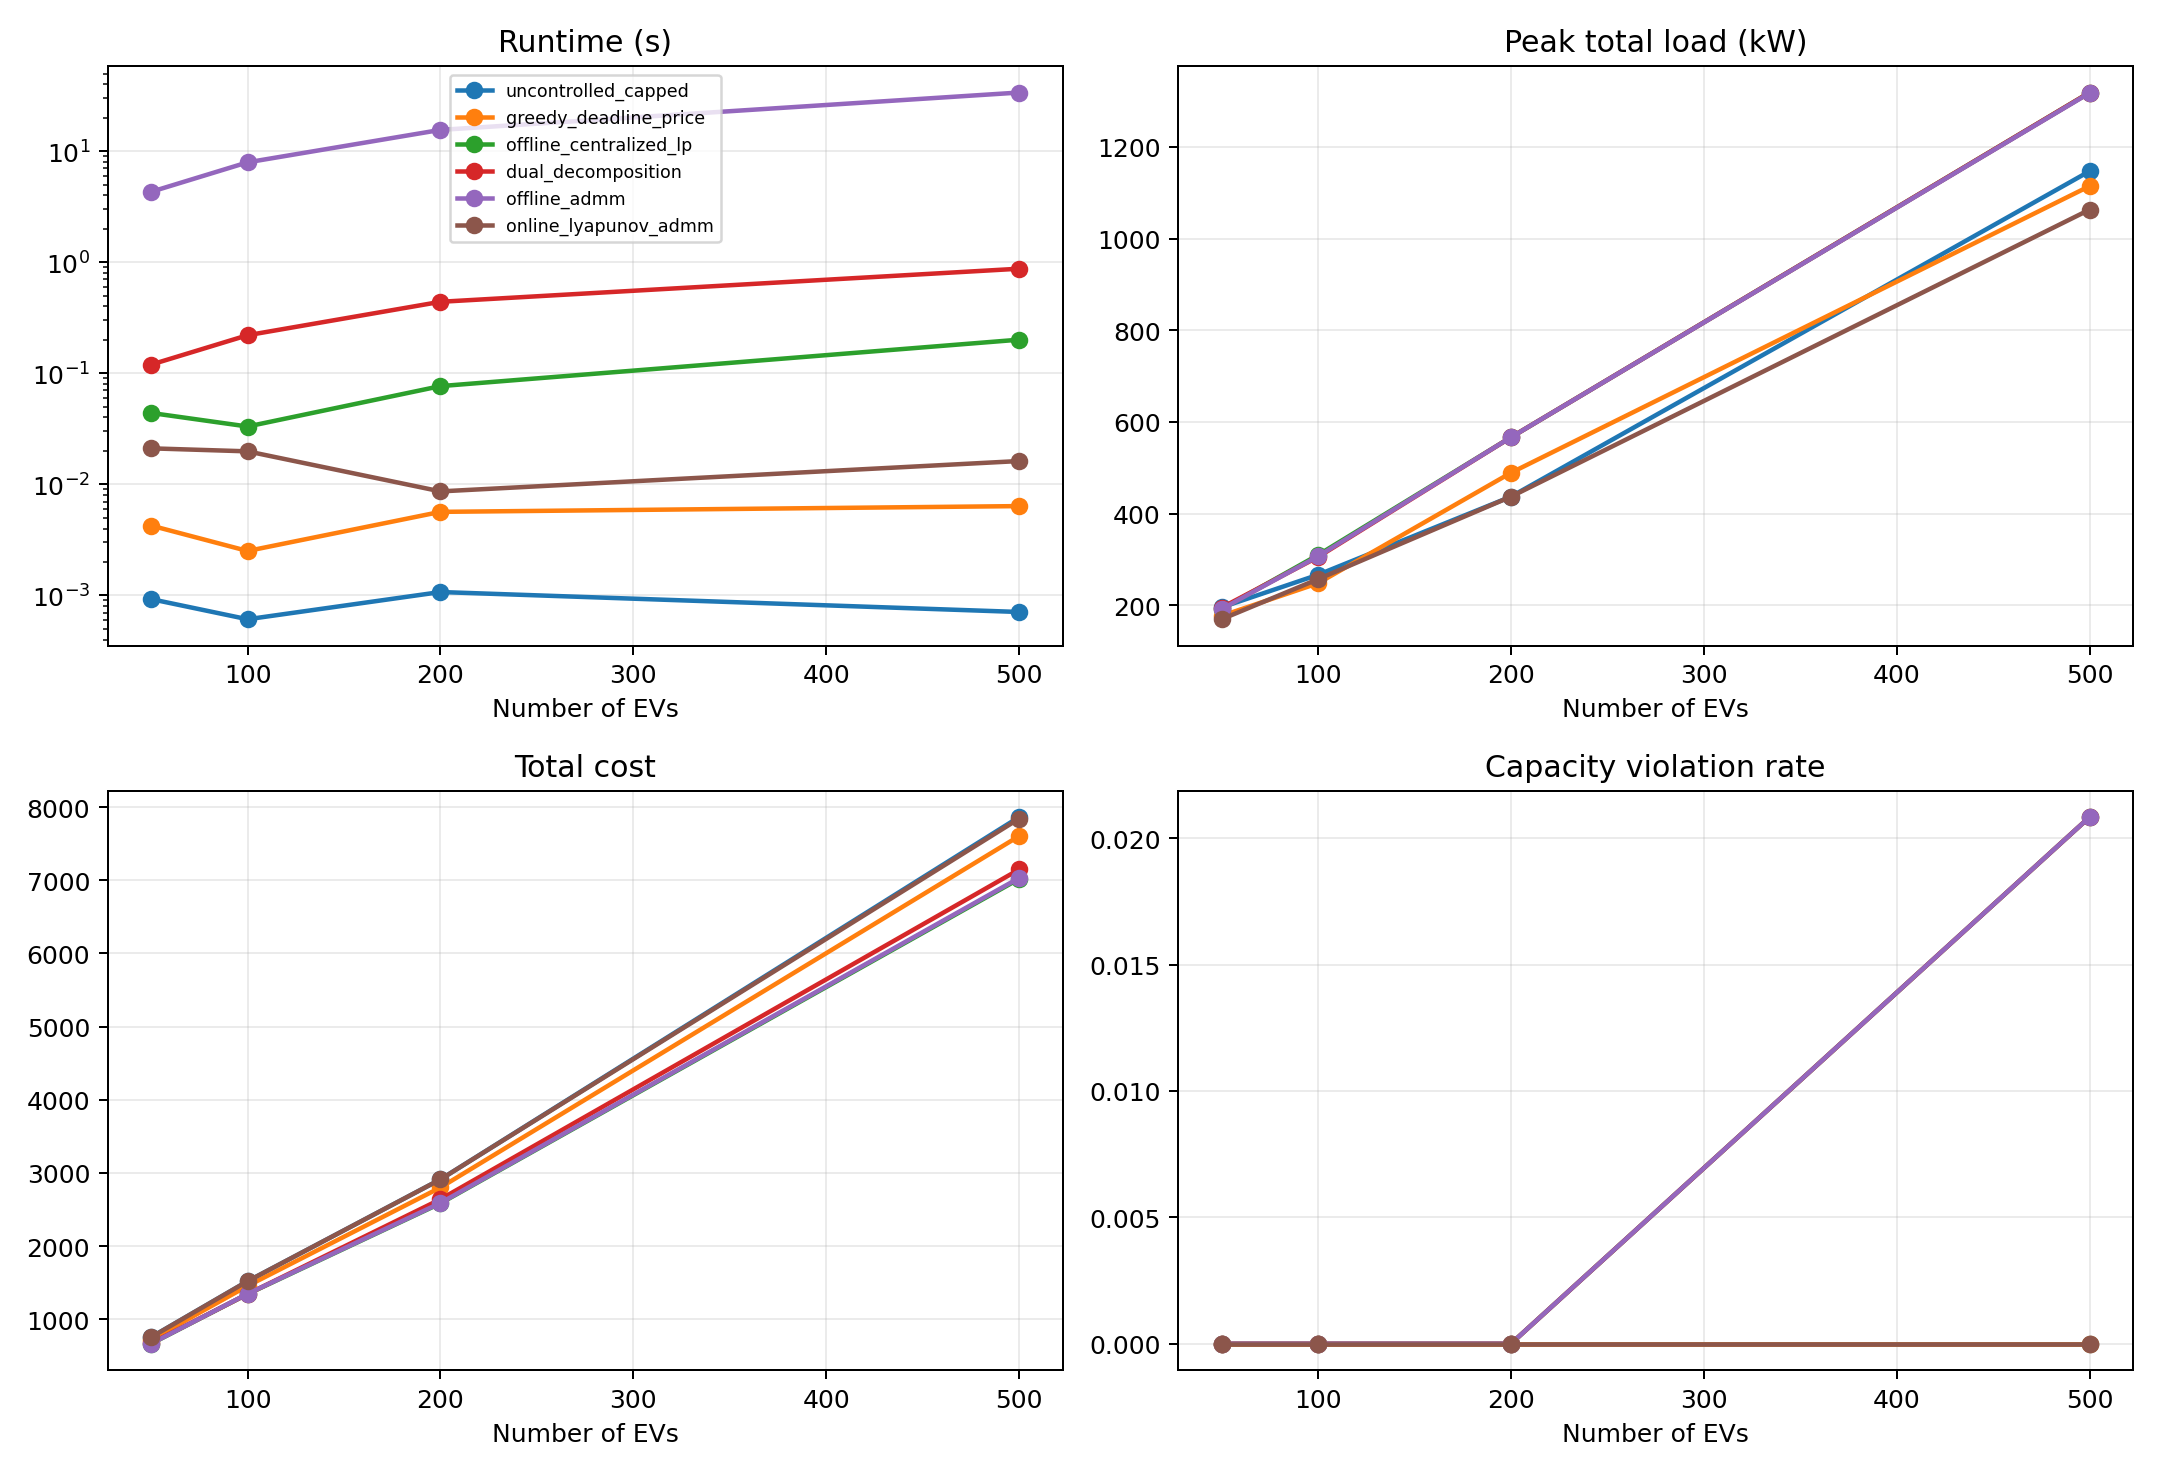
\includegraphics[width=0.95\linewidth]{../outputs/scalability_sweep_with_baselines/scalability_sweep_summary.png}
\caption{Scalability sweep from 50 to 500 EVs. Offline ADMM runtime grows substantially, while online Lyapunov-ADMM remains fast because it solves per-slot online problems.}
\label{fig:scalability}
\end{figure}

Fig.~\ref{fig:scalability} compares scalability. Offline ADMM becomes much slower as the number of EVs increases, reaching about 33 seconds for 500 EVs in the implemented simulation. Online Lyapunov-ADMM remains fast because it only solves the current per-slot problem instead of the whole-day scheduling problem. This supports its practical use in online charging stations.

\section{Discussion}
The experiments show that different methods serve different purposes. Offline centralized LP is valuable as a cost benchmark, but it assumes full future information and global data collection. Dual decomposition and offline ADMM demonstrate that the first-version distributed optimization idea is valid, but they still operate in an offline setting. The proposed online Lyapunov-ADMM method is more conservative in cost, but it better controls peak load and capacity risk under online uncertainty.

The method also has limitations. The experiments use synthetic charging scenarios rather than real charging-station data. The risk model uses a simple safety margin instead of a full chance-constrained formulation. Battery degradation, vehicle-to-grid operation, renewable generation uncertainty, and asynchronous communication are not considered. These limitations define clear directions for future work.

\section{Conclusion}
This paper proposed an online risk-aware distributed EV charging framework that combines deadline-aware virtual queues, Lyapunov drift-plus-penalty control, and ADMM-based per-slot coordination. Numerical experiments show that offline optimization achieves lower charging cost when future information is available, while the proposed online Lyapunov-ADMM method provides lower peak load, strong deadline satisfaction, better capacity safety, and scalable online computation. Future work will evaluate the method on real charging datasets and extend the model to battery degradation, renewable uncertainty, and asynchronous distributed implementation.

\bibliographystyle{IEEEtran}
\bibliography{references}

\end{document}
